\section{$PSF$ approximation for fast and distributed deconvolution} \label{gradients}
This section describes our main hypothesis of this work: Our hypothesis is that we can approximate the $PSF$ in the deconvolution problem and exploit it to speed up/distribute the deconvolution.

Our reasoning for the hypothesis comes from the Major/Minor cycle architecture. The major cycle calculates the dirty image from the visibilities. The dirty image is the product of the observed image convolved with the $PSF$ of the instrument. The deconvolution algorithm assumes the $PSF$ is constant over the image, but modern interferometers have a $w$-term, which changes the $PSF$ depending on the pixel. This is why we need the major cycle. After a number of Minor cycles (iterations of the deconvolution algorithm), we use the Major cycle to correct for the errors we introduced with the constant $PSF$. The Major cycle allows us to use an approximate $PSF$ in the deconvolution problem. We believe this can be exploited to speed up/distribute the deconvolution.

\begin{figure}[h]
	\centering
	\begin{subfigure}[b]{0.245\linewidth}
		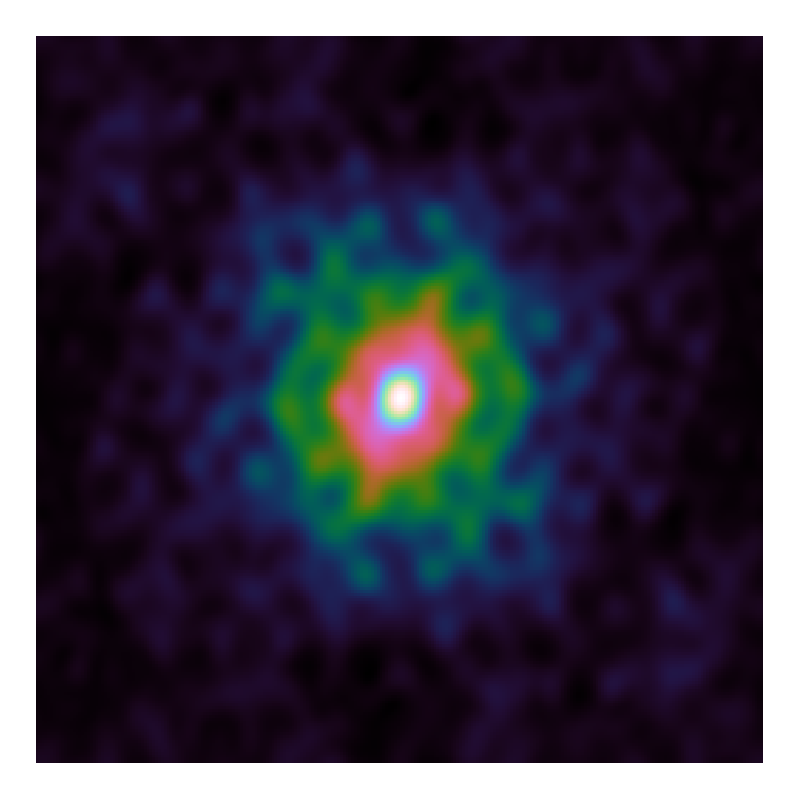
\includegraphics[width=\linewidth, clip, trim= 0.25in 0.25in 0.25in 0.25in]{./chapters/03.cd/simulated/psf.png}
		\caption{Full $PSF$}
	\end{subfigure}
	\begin{subfigure}[b]{0.245\linewidth}
		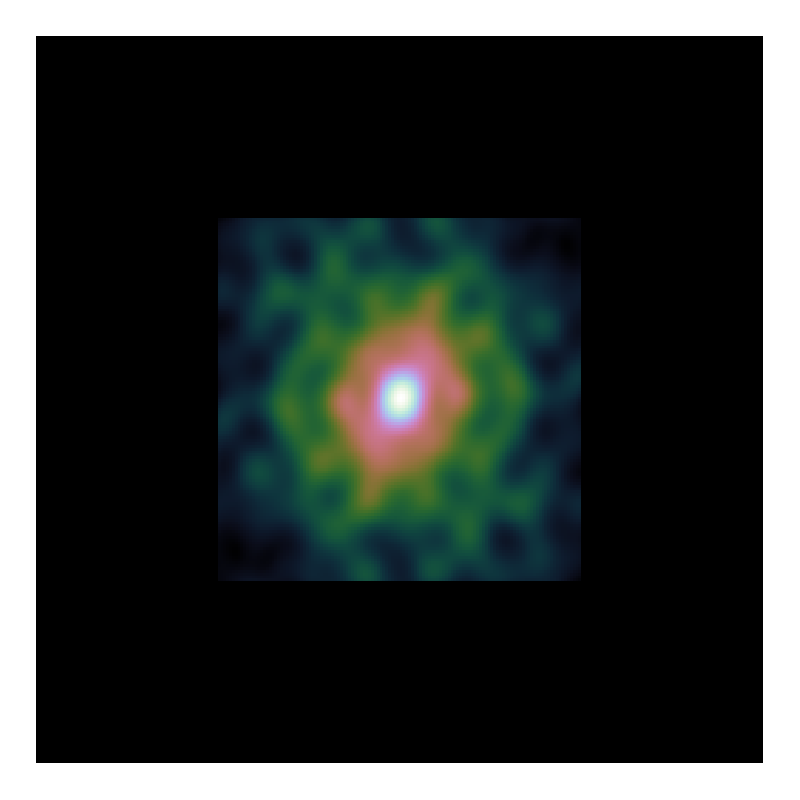
\includegraphics[width=\linewidth, clip, trim= 0.25in 0.25in 0.25in 0.25in]{./chapters/03.cd/simulated/psfCut.png}
		\caption{$\frac{1}{2}PSF$ approximation}
	\end{subfigure}
	\caption{$PSF$ approximation typically used in Clark CLEAN}
	\label{gradients:clark}
\end{figure}

A similar idea has been in use in CLEAN for decades. The Clark CLEAN algorithm \cite{clark1980efficient}. Uses only a window of the $PSF$ for the deconvolution. Figure \ref{gradients:clark} shows the full $PSF$ and the approximate $PSF$ used typically in Clark CLEAN. During deconvolution, it only uses a window around the center of the full $PSF$. Typically, the sides of the window is $\frac{1}{2}$ of the image size. By using only a $\frac{1}{2} PSF$ window around the center, a Clark CLEAN iteration is significantly faster than standard CLEAN. With $\frac{1}{2} PSF$, Clark CLEAN has to subtract only the $\frac{1}{2} PSF$ window from the residuals, which is 4 times smaller than the full $PSF$.

Using only a fraction fo the true $PSF$ speeds up the deconvolution. But it also introduces sparsity in the deconvolution problem which, to our knowledge, has not been explored for radio interferometers. The full $PSF$ shown in Figure \ref{gradients:clark} has significant values around the center, but they quickly approach zero the further away we move from the center. If we only use a window around the center $\frac{1}{2} PSF$ and set the rest to zero, we are using a sparse $PSF$. For a CLEAN algorithm, the sparse approximated $PSF$ ignores the influence of far away pixel. If we increase the approximation, the deconvolution problem becomes increasingly separable into image facets. With a $\frac{1}{8} PSF$, we can split the image into 16 facets, 4 of which are independent from each other. This problem can be easily distributed onto 4 nodes, each deconvolving an independent facet in parallel.

The important question is, how small can the center window be? Can we guarantee that the algorithm converges to the same solution, even with an approximated $PSF$? We will test the effect of an approximate $PSF$ with our serial coordinate descent algorithm  on a real-world observation in Section \ref{results:gradients}. In this section, we show how we can incorporate an approximate $PSF$ into our serial coordinate descent algorithm.


\subsection{$PSF$ approximation for the serial coordinate descent algorithm}
The serial coordinate descent algorithm keeps the gradient map, the product $PSF \star PSF$ and the current reconstruction in memory. In each iteration, the algorithm first finds the pixel, which has the maximum possible difference in this iteration. In the second step, it subtracts the product $PSF \star PSF$ at the correct location of the gradient map. The gradient map is now updated for the next iteration of the serial coordinate descent algorithm. 

We approximate the $PSF$ by only using a window around the center. Each side is only a fraction of the full $PSF$ size. From now on, we use the method $Cut()$, which cuts out the center window of the $PSF$. If we use a cut fraction of $\frac{1}{4}$, we cut out a window of the $PSF$, each side being  $\frac{1}{4}$ the length of the full $PSF$.

Using an approximate $PSF$ influences three parts of the algorithm: The gradient map, the Lipschitz map and the product $PSF \star PSF$. At the beginning of the algorithm, we calculate the gradient map by correlating the dirty image with the $PSF$ ($I_{dirty} \star PSF$) We also calculate the Lipschitz constants for each pixel. The product $PSF \star PSF$ is used to update the gradient map in each iteration. We developed two approximation methods for the serial coordinate descent algorithm. Method 1 is called 'approximate update', and method 2 is called 'approximate deconvolution'. 

\subsubsection{Method 1: Approximate update}
The approximate update method only uses the approximate $PSF$ for updating the gradient map. Instead of using the product $PSF \star PSF$, this method uses the product $Cut(PSF) \star Cut(PSF)$ to update the gradient map in each iteration. Figure \ref{gradients:update:figure} shows the effect of the approximation.  

\begin{figure}[h]
	\centering
	\begin{subfigure}[b]{0.245\linewidth}
		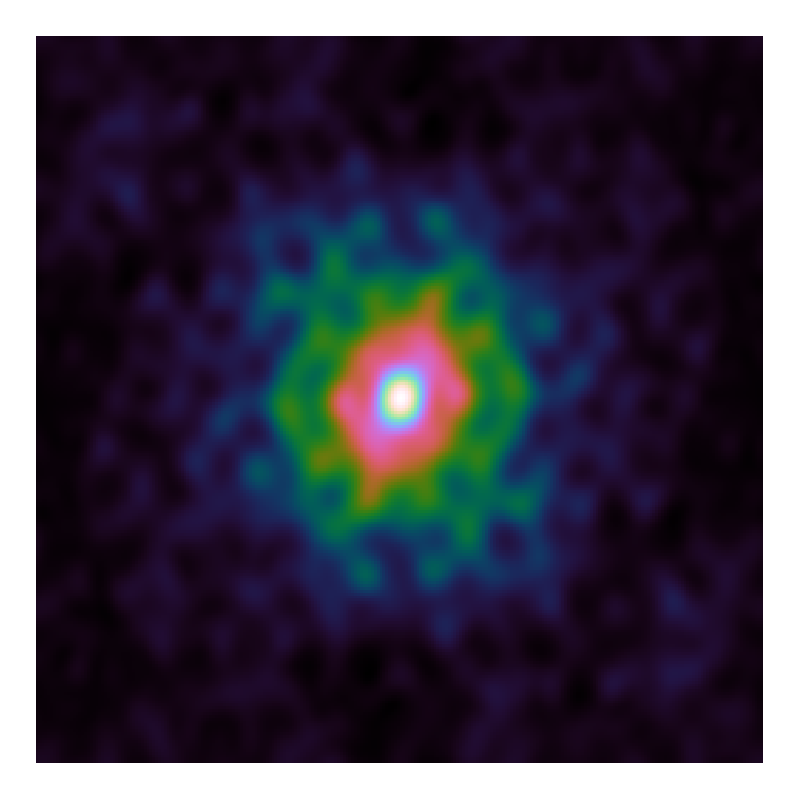
\includegraphics[width=\linewidth, clip, trim= 0.25in 0.25in 0.25in 0.25in]{./chapters/03.cd/simulated/psf.png}
		\caption{$PSF$}
	\end{subfigure}
	\begin{subfigure}[b]{0.245\linewidth}
		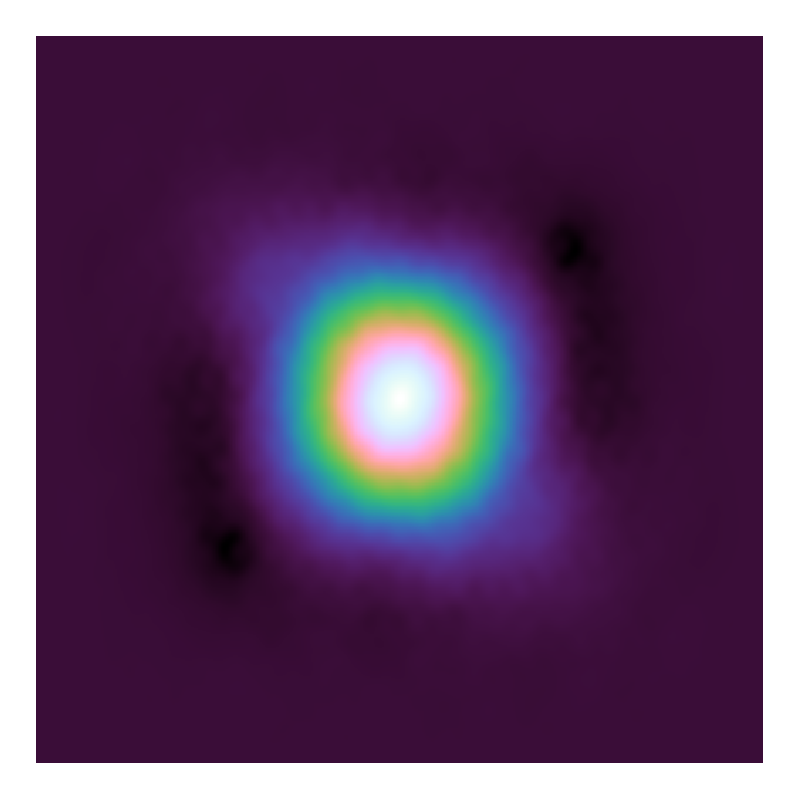
\includegraphics[width=\linewidth, clip, trim= 0.25in 0.25in 0.25in 0.25in]{./chapters/03.cd/simulated/psfSquared.png}
		\caption{Gradient update}
	\end{subfigure}
	\begin{subfigure}[b]{0.245\linewidth}
		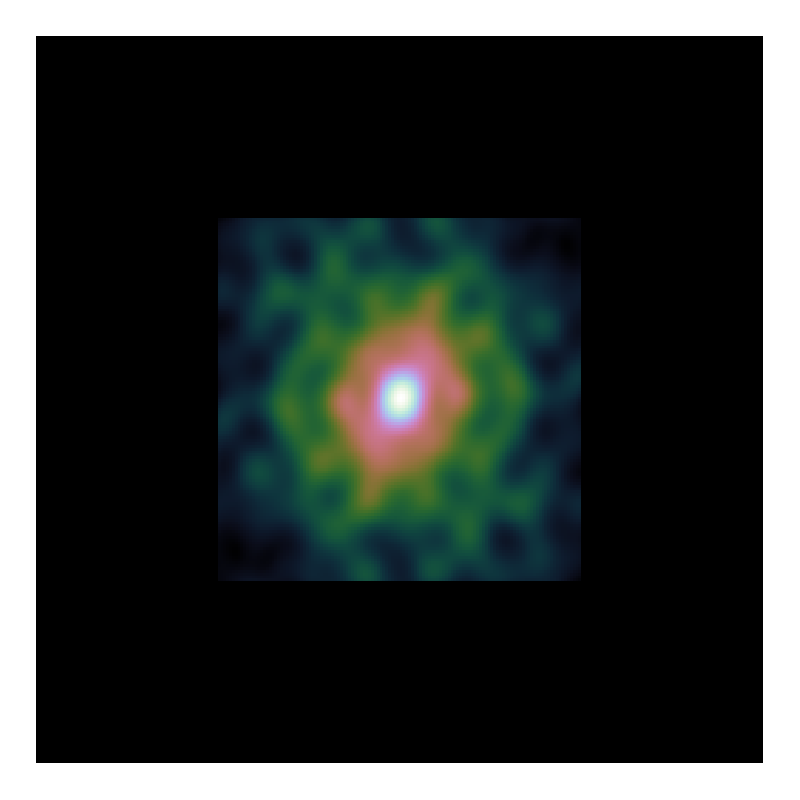
\includegraphics[width=\linewidth, clip, trim= 0.25in 0.25in 0.25in 0.25in]{./chapters/03.cd/simulated/psfCut.png}
		\caption{$Cut(PSF)$}
	\end{subfigure}
	\begin{subfigure}[b]{0.245\linewidth}
		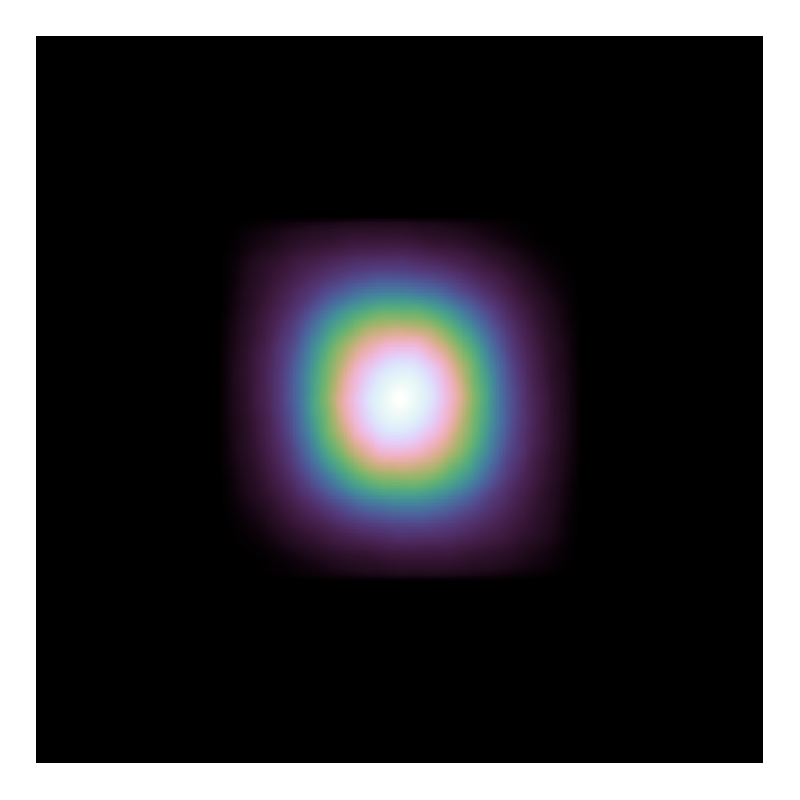
\includegraphics[width=\linewidth, clip, trim= 0.25in 0.25in 0.25in 0.25in]{./chapters/03.cd/simulated/psfSquaredCut.png}
		\caption{Approx. update}
	\end{subfigure}
	
	\caption{Approximation of gradient update.}
	\label{gradients:update:figure}
\end{figure} 

This method uses the full $PSF$ to initialize the gradient and the Lipschitz map. But it only uses an approximation for the update in each iteration of serial coordinate descent. The error we introduce with the approximation gets more severe with more iterations of serial coordinate descent. But the upside is the first iteration in every Major cycle is always identical to the serial coordinate descent algorithm without approximation. This means with enough major cycles, we are guaranteed to converge to the same result.


\subsubsection{Method 2: Approximate deconvolution}
This method also uses the approximate gradient update. But instead of initializing the gradient map with the full $PSF$, it also uses the approximate $PSF$ for initializing the gradient and the Lipschitz map. In essence, this method solves an approximate deconvolution problem:

\begin{equation}\label{gradients:method2:objective}
\underset{x}{minimize} \: \frac{1}{2} \left \| I_{dirty} - x * Cut(PSF) \right \|_2^2 + \lambda ElasticNet(x)
\end{equation}

This method does not introduce an error in every serial coordinate descent iteration. But it comes with the downside: It is not guaranteed to converge to the same result as the serial coordinate descent without approximation. It systematically under-estimates the pixel values in the reconstructed image.

To combat the under-estimation of pixel values, we reduce the regularization parameter $\lambda$ for the approximate deconvolution problem. Since we cut off parts of the $PSF$, we also reduce the Lipschitz constant (sum of the squared $PSF$ values) used in the approximate deconvolution. We reduce the $\lambda$ parameter by the same factor that the Lipschitz constant gets reduced. This ensures that the approximate deconvolution and the original deconvolution arrive at the same pixel value for a point source in theory. But it does not completely remove the issue for extended emissions.


\subsubsection{Combining the two approximation methods}
The two approximation methods developed here have opposing downsides: Method 1 is guaranteed to converge to the same result, given enough major cycles, but becomes increasingly inaccurate with more serial coordinate descent iterations. Method 2 does not become increasingly inaccurate, but is not guaranteed to converge to the same result, even with an infinite number of Major cycles.

The obvious question is, what happens when we combine the two approximation method. Indeed, this is our final solution in this project. We start out with method 2, the approximate deconvolution for a few Major cycles, and then switch to method 1, approximate update. When combining both methods, we decided to switch from method 2 to method 1 when the serial coordinate descent has converged.


\subsection{Major Cycle convergence and implicit path regularization}\label{gradients:pathreg}
There is one problem with the approximate $PSF$ which is left to solve: When does the serial coordinate descent algorithm decide to use a Major cycle. Or when we combine the $PSF$ approximation methods, how many Major cycles do we use for each method?

When we use an approximate $PSF$, the deconvolution algorithm will at a certain iteration start to include 'side lobes' of the $PSF$. The Figure \ref{gradient:convergence:sidelobe} shows an example of the side lobes we introduce by approximating the $PSF$ with $\frac{1}{2}$ of the center window. At a certain point, the deconvolution with an approximate $PSF$ has to decide whether the emission is real, or whether it is an artifact from the $PSF$ approximation, and will be removed with the next major cycle.

%re-introduce residuals

\begin{figure}[h]
	\centering
	\begin{subfigure}[b]{0.3\linewidth}
		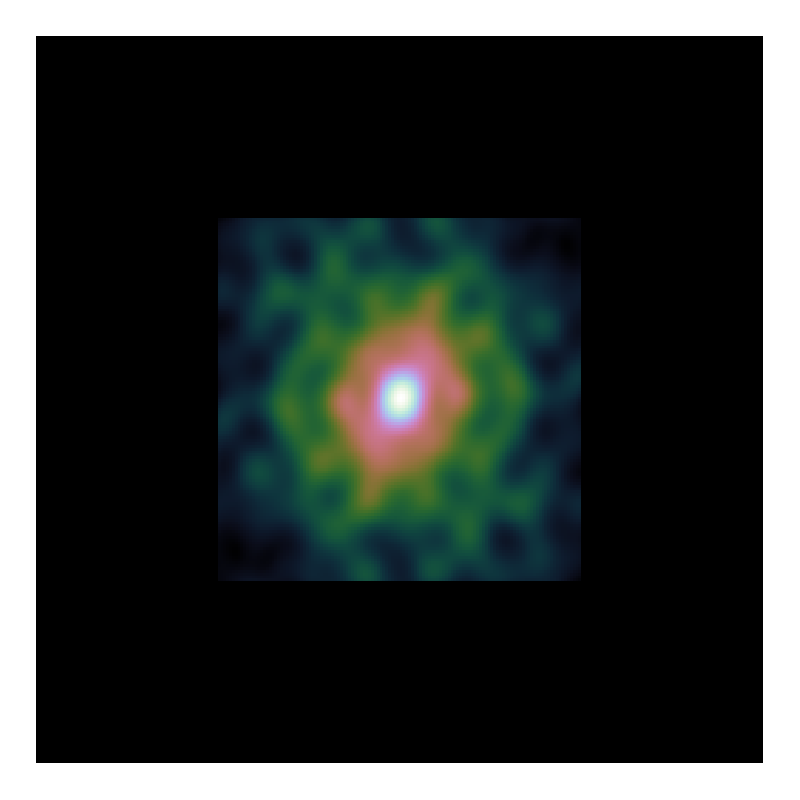
\includegraphics[width=\linewidth, clip, trim= 0.25in 0.25in 0.25in 0.25in]{./chapters/03.cd/simulated/psfCut.png}
		\caption{$\frac{1}{2}PSF$ approximation}
	\end{subfigure}
	\begin{subfigure}[b]{0.3\linewidth}
		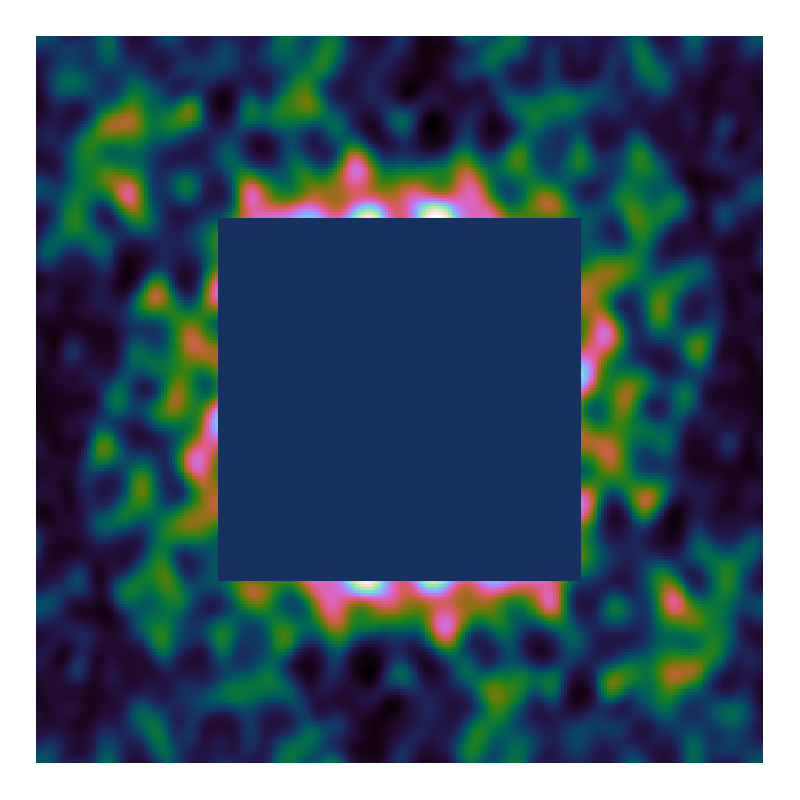
\includegraphics[width=\linewidth, clip, trim= 0.25in 0.25in 0.25in 0.25in]{./chapters/03.cd/simulated/psfReverseCut.png}
		\caption{$PSF$ Sidelobes}
		\label{gradient:convergence:reverseCut}
	\end{subfigure}
	
	\caption{Maximum sidelobe of the $PSF$ cutoff.}
	\label{gradient:convergence:sidelobe}
\end{figure}

For example: if we have an observation with a single point source in the center, the first iteration of Clark CLEAN will subtract the approximate $PSF$ from the residuals. But the residual image is left with the $PSF$ side lobes shown in Figure \ref{gradient:convergence:reverseCut}. The next iteration may detect 'fake' point sources at the significant side lobes of the $PSF$. Our serial coordinate descent algorithm does not explicitly use the residual image, but has a similar problem. The information of the residual image is implicitly contained in the gradient map. Our serial coordinate descent algorithm with an approximate $PSF$ leaves significant gradients in the map.

This is a problem for deconvolving an image with the Major cycle. If we let our serial coordinate descent algorithm converge to a result in each Major cycle, it will include emission from the $PSF$ side lobes. In the next Major cycle, the serial coordinate descent algorithm has to remove the side lobes from the reconstruction, but this again leaves significant side lobes in the gradient map. This can lead to an oscillation of the algorithm, where it adds and removes the same side lobes several times over different Major cycles. In extreme cases (for example when we use an aggressive approximation of the $PSF$), this may even lead to a diverging behavior. But even if the deconvolution algorithm converges over several Major cycles, if the algorithm spends too much time on $PSF$ side lobes, it may become significantly slower.

To solve this problem, we use the following strategy for our serial coordinate descent algorithm: We estimate the $PSF$ side lobes introduced by the approximation. We increase the regularization parameter $\lambda$, until the elastic net regularization excludes all side lobes from the reconstruction. Note that real emission may also be regularized away in the current Major cycle iteration. The serial coordinate descent algorithm reconstructs the image with the current $\lambda$, and lets the Major cycle remove the side lobes. It then estimates the current $PSF$ side lobes for this Major cycle, sets a lower regularization parameter $\lambda$ and again deconvolves the image.

This is known as a path regularization in optimization. We let our optimization algorithm converge on intermediate solution, decrease the $\lambda$ parameter and use the intermediate solution as a 'warm start'. Coordinate descent methods may benefit from path regularization\cite{friedman2010regularization}. Converging on all intermediate solutions may result in a lower wall-clock time than converging directly on the final solution.

We use the path regularization to stop the algorithm from wasting computing resources on side lobes. There may be different strategies that result in an overall lower wall-clock time for the serial coordinate descent algorithm, but they were not explored in this project. We set the regularization parameter $\lambda$ for each Major cycle according to the following estimate:

\begin{equation}
\begin{split}
maxSidelobe &= Max(PSF - Cut(PSF)) \\
gradients &= residuals \star PSF \\
maxLobeGradient &= Max(gradients) * maxSidelobe \\
\lambda_{cycle} &= \frac{maxLobeGradient}{\alpha}\\
\lambda_{cycle} &= Max(\lambda, \lambda_{cycle})
\end{split}
\end{equation}

We calculate the maximum side lobe of the $PSF$ approximation. We then multiply the maximum side lobe with the maximum gradient. This is an estimate of the largest gradient value, which gets left in the gradient map by the $PSF$ approximation. We then set the $\lambda_{cycle}$ parameter to exclude all gradients equal or smaller that gradient magnitude. The maximum of the gradient map decreases over every Major cycle, which leads to a decreasing $\lambda_{cycle}$ until we reached the target value $\lambda$.

This estimate works, but it has one problem for radio interferometric imaging: It does not account for extended emissions. Since they have non-zero pixel values close to each other, their $PSF$ side lobes also overlap. Meaning the $PSF$ side lobes of extended emissions are higher than we estimated. This is why we added a correction factor which estimates how much the maximum in the gradient map is point-source-like:

\begin{equation}
\begin{split}
maxSidelobe &= Max(PSF - cut(PSF)) \\
gradients &= residuals \star PSF \\
\textbf{correction} &= Max(1, \frac{Max(gradients)}{Max(residuals) * Lipschitz}) \\
maxLobeGradient &= Max(gradients) * maxSidelobe * correction \\
\lambda_{cycle} &= \frac{maxLobeGradient}{\alpha}\\
\lambda_{cycle} &= Max(\lambda, \lambda_{cycle})
\end{split}
\end{equation}

It the same estimate as before, except for the correction factor. The correction factor is 1 if the maximum in the gradient map is a point source, and $1 <$ if the maximum in the gradient map is more like an extended emission. The correction factor is based on the following observation: If the image only contains point sources, then the maximum of the gradient map should be equal the maximum of the residuals times the Lipschitz constant. But if it is an extended emission, the maximum of the gradient map will be significantly larger.


T

In the two presented methods, we use a fraction of the $PSF$ to approximate the deconvolution problem. Both methods rely on the Major Cycle to periodically reset the gradient map. By using only a fraction of the $PSF$, the approximate deconvolution leaves parts of the $PSF$ in the gradient map. Figure \ref{gradient:convergence:sidelobe} shows the fraction of the $PSF$ that get included in the deconvolution, and "sidelobes" which get ignored.




The basic coordinate descent method first correlates the residuals with the $PSF$. It pre-calculates the gradient for each pixel. Then, in each iteration, it directly updates the map of gradients with the product of $PSF \star PSF$ (the $PSF$ correlated with itself). In this approximation method, we start from the same pre-calculated map of gradients, but use an approximate update. The first coordinate descent iteration of this approximation method is identical to coordinate descent with the full $PSF$. With each coordinate descent iterations, the gradient map becomes more inaccurate. But with enough major cycles, this method converges to the same result as when the full $PSF$ is used.

The question is, how do we approximate the product of $PSF \star PSF$. As we have seen before, the product of $PSF \star PSF$ also approaches zero away from the center (an example was shown in Figure \ref{cd:efficient:update:figure} in Section \ref{cd:efficient:update}). A naive way to approximate the update step is to cut off the insignificant value and only use a rectangle of the center, which is a fraction of the total image size. For example: An image of size $1024^2$ also has a $PSF$ the size of $1024^2$. The product $PSF \star PSF$ actually has the size of $2048^2$ pixels due to the correlation. We can try to approximate the product by only using the center rectangle $\frac{1}{8}$ of the total size, ($256^2$ pixels). This approximation works, but leads to artifacts during deconvolution: The image will be reconstructed in visible "blocks" which are the size of the center fraction we use. 

We use the approximation shown in equation \eqref{gradient:method1:psf2}, where $cut()$ is the function that cuts away everything but the center rectangle of the $PSF$. This is a better approximation than cutting the product of $PSF \star PSF$ directly, and leads to faster convergence.

\begin{equation}\label{gradient:method1:psf2}
PSF \star PSF \approx cut(PSF) \star cut(PSF)
\end{equation}

The reason why \eqref{gradient:method1:psf2} is a better approximation lies in the reason why we update the gradients with the product of $PSF \star PSF$ in the first place: It is the combination of two separate operations, removing the $PSF$ from the residuals at the current position, and recalculating the correlation with the $PSF$. If we cut away parts of the product $PSF \star PSF$ directly, we implicitly update the residuals with a different $PSF$. But when we approximate the product by \eqref{gradient:method1:psf2}, we ensure that the implicit removal of the $PSF$ from the residuals is equal to $cut(PSF)$.

In our implementation, we use one more trick to improve the approximation: we scale the product of $cut(PSF) \star cut(PSF)$ to have the same maximum as the original product $PSF \star PSF$. The approximation has a lower maximum value than the original. Over several coordinate descent iterations, we run into the danger of over-estimating the pixel values. By scaling the product of $cut(PSF) \star cut(PSF)$ to the same maximum, we end up with a better approximation of the true gradient update.

\subsection{Method 2:Approximate deconvolution}
\begin{figure}[h]
	\centering
	\begin{subfigure}[b]{0.3\linewidth}
		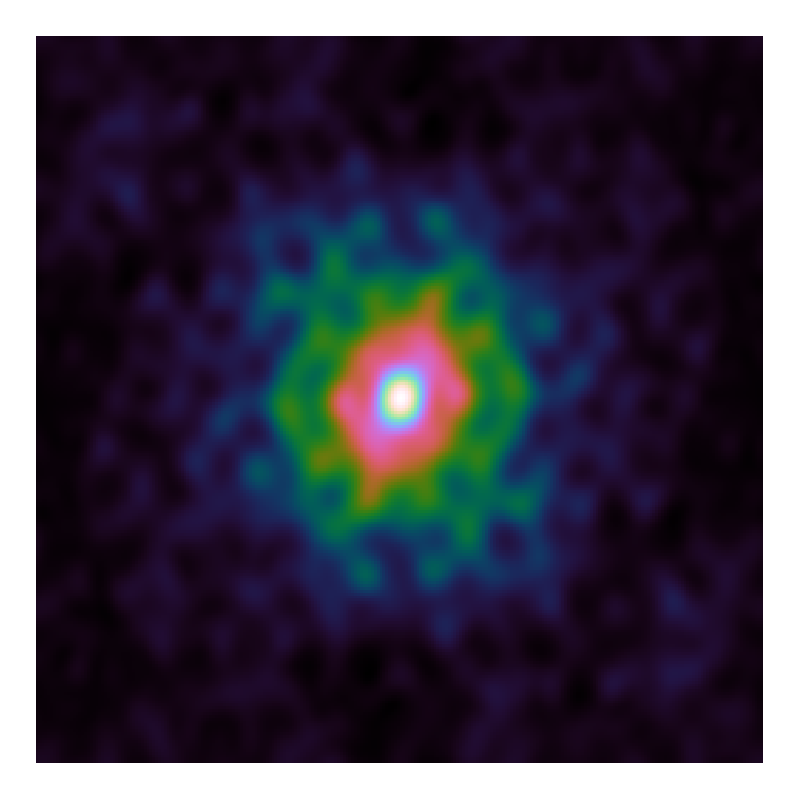
\includegraphics[width=\linewidth, clip, trim= 0.25in 0.25in 0.25in 0.25in]{./chapters/03.cd/simulated/psf.png}
		\caption{$PSF$ on log scale}
	\end{subfigure}
	\begin{subfigure}[b]{0.3\linewidth}
		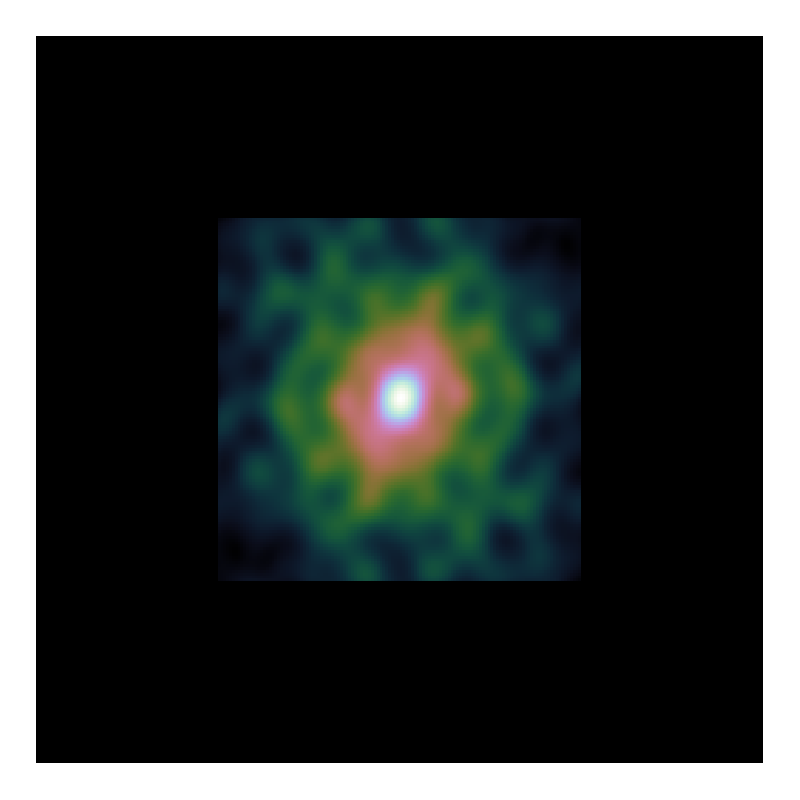
\includegraphics[width=\linewidth,clip, trim= 0.25in 0.25in 0.25in 0.25in]{./chapters/03.cd/simulated/psfCut.png}
		\caption{$\frac{1}{2}$ Fraction of the $PSF$}
	\end{subfigure}
	
	\caption{Approximate deconvolution with fraction $\frac{1}{2}$ of the $PSF$.}
\end{figure} 
The main problem with Method 1 is that the map of gradients becomes less accurate with more coordinate descent iterations. This method sovles this problem by using an approximate deconvolution instead, but it loses the guarantee to converge to the same result as the full $PSF$.

This method cuts off the insignificant part of the $PSF$, and only uses the center rectangle of it for the whole deconvolution problem. As such, the coordinate descent method solves an approximate deconvolution problem shown in \eqref{gradients:method2:objective}.

\begin{equation}\label{gradients:method2:objective}
\underset{x}{minimize} \: \frac{1}{2} \left \| I_{dirty} - x * cut(PSF) \right \|_2^2 + \lambda ElasticNet(x)
\end{equation}

In essence, it uses the same basic coordinate descent method, but ignore large parts of the $PSF$. It pre-calculates the gradient map by correlating the residual image with $cut(PSF)$, and update the gradient map with the product of $cut(PSF) \star cut(PSF)$. The main difference between approximate gradient update and approximate deconvolution is: In approximate gradient update starts with the same gradient map as the original. The approximate deconvolution does not. With this method, the gradient map does not become more inaccurate with more coordinate descent iterations.

The approximate deconvolution objective \eqref{gradients:method2:objective} is not guaranteed to "point" to the same solution as the original. It may in reality point to a very different solution. But thanks to the Major cycle, the image retrieved by optimizing \eqref{gradients:method2:objective} is always "close" to the original solution.

Nevertheless, this approximation method introduces an error in the final reconstructed image. The obvious error it introduces is it under-estimates the true pixel values. Pre-calculating the gradient map with $cut(PSF)$ under-estimates gradient magnitudes, and by extend the pixel values.

To combat the under-estimation of pixel values, we reduce the regularization parameter $\lambda$ for the approximate deconvolution problem. Since we cut off parts of the $PSF$, we also reduce the Lipschitz constant (sum of the squared $PSF$ values) used in the approximate deconvolution. We reduce the $\lambda$ parameter by the same factor that the Lipschitz constant gets reduced. This ensures that the approximate deconvolution and the original deconvolution arrive at the same pixel value for a point source. But it does not completely remove the issue for extended emissions.

\subsection{Major Cycle convergence and implicit path regularization}\label{gradients:pathreg}
In the two presented methods, we use a fraction of the $PSF$ to approximate the deconvolution problem. Both methods rely on the Major Cycle to periodically reset the gradient map. By using only a fraction of the $PSF$, the approximate deconvolution leaves parts of the $PSF$ in the gradient map. Figure \ref{gradient:convergence:sidelobe} shows the fraction of the $PSF$ that get included in the deconvolution, and "sidelobes" which get ignored.

%re-introduce residuals

\begin{figure}[h]
	\centering
	\begin{subfigure}[b]{0.3\linewidth}
		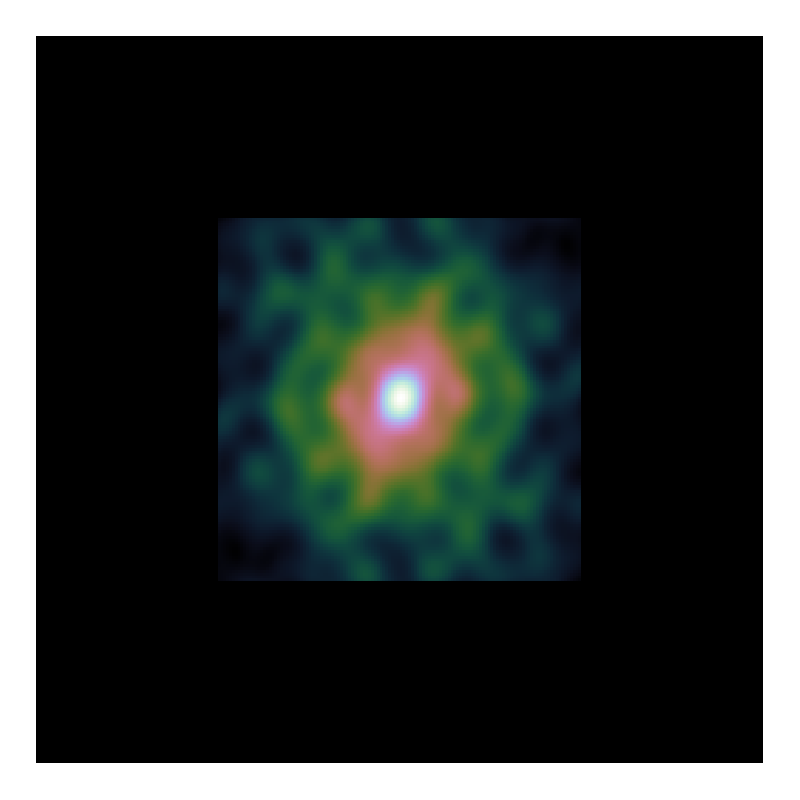
\includegraphics[width=\linewidth, clip, trim= 0.25in 0.25in 0.25in 0.25in]{./chapters/03.cd/simulated/psfCut.png}
		\caption{$\frac{1}{2}$ Fraction of the $PSF$}
	\end{subfigure}
	\begin{subfigure}[b]{0.3\linewidth}
		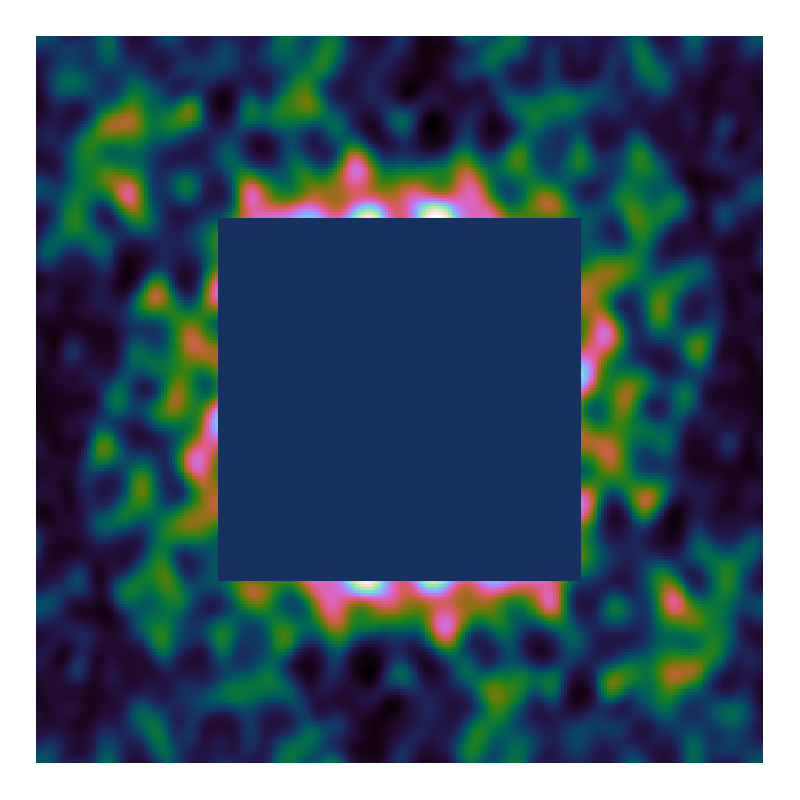
\includegraphics[width=\linewidth, clip, trim= 0.25in 0.25in 0.25in 0.25in]{./chapters/03.cd/simulated/psfReverseCut.png}
		\caption{$PSF$ Sidelobes}
		\label{gradient:convergence:reverseCut}
	\end{subfigure}
	
	\caption{Max sidelobe of the $PSF$ cutoff.}
	\label{gradient:convergence:sidelobe}
\end{figure}

After a number of serial coordinate descent iterations, we run into the danger of deconvolving the leftovers of the $PSF$ approximation. In that case, the serial coordinate descent algorithm adds spurious point sources to the image. After a major cycle, we can detect them as spurious and remove them again.
Degree to how bad this is depends on the maximum absolute value we cut off in the approximation, the maximum absolute value in Figure \ref{gradient:convergence:reverseCut}. With an aggressive approximation, we may end up oscillating from major cycle to major cycle: Adding spurious pixels and removing them again in the next, just to add the same spurious pixels in the one after.

But we can estimate at what point we are likely to add spurious pixels. This lets us estimate a minimum $\lambda$ parameter for the elastic net regularization. At this major cycle iteration, we cannot go below the minimum lambda. The next major cycle, the maximum residual is lower, and so is the minimum $\lambda$

This is known as a path regularization. We start with a stronger regularization and continually reduce $\lambda$ until we reached the desired value. We have intermediate results in each major cycle. Coordinate descent methods tend to be faster from a warm start, when we start from an intermediate result \cite{friedman2010regularization}. 

In this work we use the path regularization mainly for convergence of the major cycle. 

How we estimate the minimum $\lambda$ parameter. Imagine the interferometer only observed a point source in the center of the image. In that case, 
after the first serial coordinate descent iteration, our residuals image looks exactly like the Figure \ref{gradient:convergence:reverseCut}. The serial coordinate descent algorithm should not take another step, or it adds spurious pixels. In other words, the regularization has to suppress all the values in Figure \ref{gradient:convergence:reverseCut}

Remember the elastic net regularization: It is a mixture of the L1 and L2 norm. The L1 norm shrinks the pixel values, while the L2 norm divides them. We need the L1 norm to shrink away the values in Figure \ref{gradient:convergence:reverseCut}.

\begin{equation}
\begin{split}
gradients &= residuals \star PSF \\
maxSidelobe &= Max(gradients) * Max(Abs(Sidelobe(PSF)))) \\
\lambda_{cycle} &= \frac{maxSidelobe}{\alpha}
\end{split}
\end{equation}

This estimate is a minimum. Meaning it is possible that we still add spurious pixels. For example when the sidelobes of two point sources overlap.

The estimate however only considers point sources. For extended emissions, the estimate is too low. Extended emissions are a group of non-zero pixels. Beause they are next to each other, their sidelobes overlap and get amplified. 

An estimate considering extended emissions.

\begin{equation}
\begin{split}
psfSidelobe &= Max(PSF - cut(PSF)) \\
gradients &= residuals \star PSF \\
correction &= Max(1, \frac{Max(gradients)}{Max(residuals) * lipschitz}) \\
maxSidelobe &= Max(gradients) * Max(psfSidelobe) * correction \\
\lambda_{cycle} &= \frac{maxSidelobe}{\alpha}
\end{split}
\end{equation}

Only considers the "maximum" extended emission. Extended emissions tend to contain the largest pixel value in the residual image. Because of the convolution.
The correction factor gets reduced the closer the maximum pixel in the residuals. Over several major cycles, the correction factor and the $lambda_{cycle}$ become smaller. 
Helps convergence.


But this is not true for extended emissions.

he serial deconvolution algorithm calculates the gradient map (by correlating the $PSF$ with the residuals).


Residuals will be left. 



